\section{Training and scaling the decision interface}
\label{sec:train}

Having established what the representation must contain, this section asks how the interface behaves
when it is trained and scaled: typed objectives (\Cref{sec:train:typed}), the training distribution
(\Cref{sec:train:mixture}), the size ladder (\Cref{sec:train:ladder}), probability quality
(\Cref{sec:train:calibration}), and cost (\Cref{sec:train:latency}). Three runs remained in flight at
the time of writing (\texttt{ts1b\_semif}, \texttt{tl1b\_semif}, and a Qwen3.5-9B checkpoint
\texttt{tl2}) and are omitted rather than reported provisionally.

\subsection{Typed objectives are contracts on the output distribution}
\label{sec:train:typed}

The interesting result about Choice, Score, and Noul is not that they are three architectures -- they
are one backbone, one tap, and one readout -- but that one readout supports genuinely different
probabilistic semantics by changing only the target distribution and terminal head.

Matched fine-tunes (\Cref{app:typed-primitives} for full numbers) give two clean instances. Ordinal
smoothing on Score changes \emph{no} decision on JevBench's 12 ordinal items relative to plain Choice
while improving every probability-quality metric (held-out score NLL 2.07 $\to$ 1.23): a pure
calibration change, which is exactly what an ordinal contract should buy and what a relabeling could
not. The Bernoulli Noul head is exactly order-invariant by construction -- there is no candidate order
to be sensitive to -- and is the first head in this project to clear an untouched external floor by a
wide margin (PagerDuty .602 $\to$ .886 against a .792 majority-class floor).

\subsection{The training distribution controls capability}
\label{sec:train:mixture}

Adding rubric-conditioned workflow data ($W$) and the uncertainty corpus ($U$) to the
evidence/knowledge mixture without adjusting sampling ratios costs evidence accuracy (CLINC-150 $-11$,
TREC-fine $-10$ points), driven almost entirely by increased false abstention rather than lost
discrimination. A sweep of $E$ from .35 to .50 (\Cref{tab:app-mixture}) shows raising $E$ to .45--.50
restores evidence accuracy to within 1 point of an $E$-only base and intent/topic accuracy to within
3--4 points, with $W$ metrics unchanged within 1--4 points. Mixing, not architecture, caused the
regression -- and that is the general point worth carrying forward: the \emph{distribution of decision
types} is a first-order lever on capability, comparable in size to the architectural choices of
\Cref{sec:repr}.

Null augmentation ($W{:}0.20$ of workflow rows duplicated with their gold removed, target $\nullsym$)
does at the data level what a post-hoc calibration offset provably cannot do at the output level
(\Cref{sec:train:calibration}): it lowers false-abstain rates and raises MMLU-Pro accuracy to the
$E$-only base's level, with the highest $\dqsh$ of any mixture tested. The uncertainty corpus improves
likelihood (ChaosNLI NLL 1.27 $\to$ 1.00) while top-1 accuracy is flat or slightly lower, consistent
with soft targets spreading probability mass rather than sharpening it.

DecisionMix v2 moves held-out rule-grammar and rubric-style generalization sharply within the
generator's own world (\Cref{app:decisionmix}) while leaving level-7 composition at chance. We treat the
in-grammar half as an evaluation-protocol result rather than a generalization claim, since the held-out
families and the training generator share one rule engine (\Cref{tab:generalization}, rows 4--6); the
out-of-grammar half is the subject of \Cref{sec:boundary:hard}.

\subsection{The scaling ladder}
\label{sec:train:ladder}

\Cref{tab:headline} runs the identical recipe at four Qwen3 backbone sizes and once on Qwen3.5-4B,
alongside a frozen three-shot control at each size (the base model reading next-token letter logits
over the rendered options, no training at all).

\begin{table}[t]
  \centering
  \caption{Scaling ladder. \textbf{JevBench: public 231-id subset, unranked} (72 standard items over 36
  paraphrase-clustered states; 111 hard items). 95\% intervals are cluster bootstraps over the
  paraphrase \texttt{group} field, 20{,}000 resamples (\Cref{sec:experiments:jevbench}); they are wide
  and no unpaired difference smaller than them is a ranking. MMLU-$\numcands$ = MMLU-Pro
  among-$\numcands$; $\dqsh$ against a fine-tuned 1.7B teacher's own .102; latency at $\numcands{=}2$,
  same pod and build. Frozen = zero training, letter logits, 3 exemplars. Trained checkpoints:
  \texttt{ts1b}/\texttt{tm1b} (released as \texttt{typical-small}/\texttt{typical-medium}),
  \texttt{ladder\_8b}, \texttt{tl1b}, \texttt{tm2} (Qwen3.5-4B, not released).}
  \label{tab:headline}
  \small
  \setlength{\tabcolsep}{4pt}
  \begin{tabular}{lcccrrr}
    \toprule
    Model & JevBench std [95\% CI] & JevBench hard [95\% CI] & MMLU-$\numcands$ & $\dqsh$ & NLL & ms \\
    \midrule
    Qwen3-1.7B (trained) & .694 [.569, .819] & .432 [.342, .523] & .343 & .127 & 1.01 & 45 \\
    \quad frozen, 3-shot & .528 [.389, .667] & .369 [.279, .459] & -- & -- & -- & -- \\
    Qwen3-4B (trained) & .806 [.694, .903] & .423 [.333, .514] & .458 & .193 & 1.02 & 57 \\
    \quad frozen, 3-shot & .778 [.667, .889] & .441 [.351, .532] & -- & -- & -- & -- \\
    Qwen3-8B (trained) & .667 [.528, .792] & .396 [.306, .486] & .290 & .093 & 1.67 & 70 \\
    \quad frozen, 3-shot & .556 [.417, .694] & .369 [.279, .459] & -- & -- & -- & -- \\
    Qwen3-14B (trained) & \textbf{.931} [.861, .986] & .450 [.360, .541] & .486 & .235 & \textbf{0.95} & 59 \\
    \quad frozen, 3-shot & .819 [.708, .917] & \textbf{.559} [.468, .649] & -- & -- & -- & -- \\
    Qwen3.5-4B (trained) & .861 [.778, .944] & .495 [.405, .586] & .429 & .194 & 0.97 & -- \\
    \bottomrule
  \end{tabular}
\end{table}

\begin{figure}[t]
  \centering
  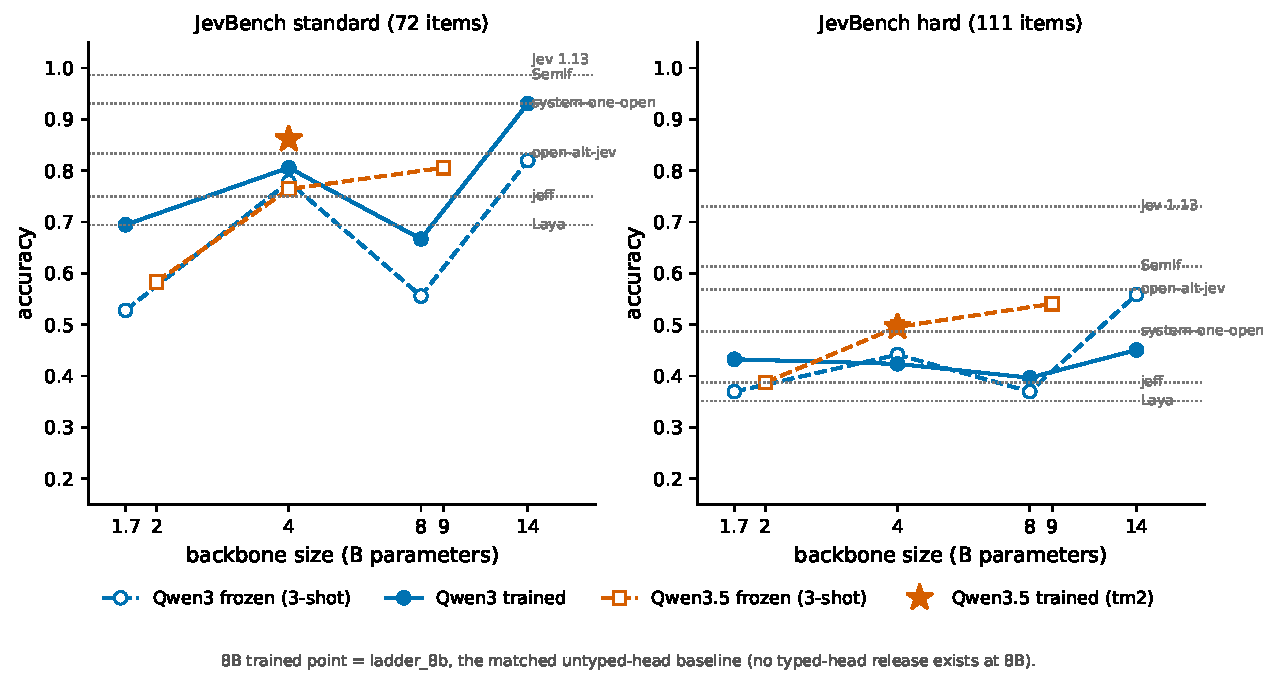
\includegraphics[width=\linewidth]{figures/fig_ladder.pdf}
  \caption{JevBench standard and hard accuracy vs.\ backbone size for Qwen3 (1.7/4/8/14B) and Qwen3.5
  (4B; 2B/9B points from frozen controls where locally available); frozen-with-3-shots dashed, trained
  solid. \textbf{Public subset, unranked}; see \Cref{tab:headline} for the intervals, which are wide.}
  \label{fig:ladder}
\end{figure}

Three readings, stated at the resolution the intervals support.

\textbf{Standard-tier performance generally improves with scale, with an anomalous 8B point.} We
deliberately do not call this monotonic and do not fit a scaling law through it: it is a scaling
\emph{ladder} of single runs. Qwen3-8B is an outlier in both frozen and trained form under the
identical recipe, and we found no tap or learning-rate setting that recovers it within budget; it should
be read as a checkpoint-specific anomaly, not as evidence about 8B-parameter backbones. Three separate
things are also being varied and should not be collapsed: backbone scale, the trained decision recipe,
and the Qwen3-vs-Qwen3.5 pretraining generation -- the single Qwen3.5-4B checkpoint reaches hard-tier
.495, above every Qwen3 checkpoint we trained at any size, at a fraction of the parameters.

\textbf{Training helps the standard tier; each individual rung is inside its interval.} The trained
model beats its frozen control on standard accuracy at all four rungs ($+16.6$, $+2.8$, $+11.1$, $+11.2$
points), which is consistent in sign at every rung, but no single rung's gap clears its own 95\%
interval, and a paired bootstrap at 14B gives $-.111$ $[-.250, +.014]$ for frozen-minus-trained
($p{=}.10$). The pattern is real; any individual number is not a measurement of its size.

\textbf{Per-decision latency is roughly flat across the ladder} (45, 57, 59\,ms at $\numcands{=}2$ for
1.7B/4B/14B), because a decision's cost is dominated by the cached-state pass and a short suffix rather
than by backbone depth (\Cref{sec:train:latency}).

The hard tier moves in the opposite direction from the standard tier and is the subject of
\Cref{sec:boundary}.

\subsection{Probability quality is trainable, and task-conditional}
\label{sec:train:calibration}

\begin{figure}[t]
  \centering
  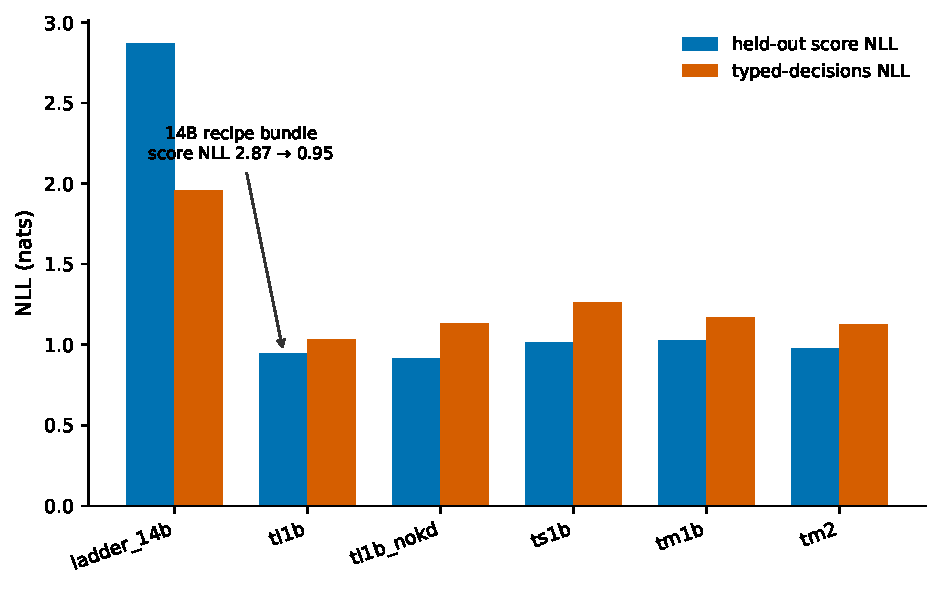
\includegraphics[width=\linewidth]{figures/fig_calibration.pdf}
  \caption{Held-out score NLL and typed-decisions NLL (held-out sets, not JevBench) across the calibration-fix sequence
  (\texttt{ladder\_14b} $\to$ \texttt{tl1b}/\texttt{tl1b\_nokd}/\texttt{ts1b}/\texttt{tm1b}/\texttt{tm2}),
  showing the 2.87 $\to$ 0.95 change in held-out soft-target likelihood at fixed backbone size.}
  \label{fig:calibration}
\end{figure}

We do not claim the model is ``calibrated''. The result we can support is more specific and more
useful: \emph{probability quality is trainable, and what a good calibration looks like is conditional on
the decision type and task family}.

\textbf{A single global knob cannot serve two regimes.} A single global temperature and null-logit
offset, fit jointly on held-out soft-target rows, moves in \emph{opposite} directions for an
evidence/knowledge-only checkpoint and a workflow-trained one. For the former it reduces false
abstention and repairs CLINC-150 (false-abstain .053 $\to$ .022); for the latter the same fitting
procedure pushes the offset to $+3.0$, which repairs typed-decisions NLL (1.95 $\to$ 1.19) but collapses
intent/topic coverage to 5--9\%. Calibration for this class of model has to be per decision-type or per
family, which is what null augmentation (\Cref{sec:train:mixture}) and per-type target distributions
(\Cref{sec:train:typed}) supply at the data and objective level instead of at the output.

\textbf{The selection criterion, not capacity, was the binding constraint.} Under an accuracy-shaped
selection criterion, held-out soft-target NLL got \emph{worse} with backbone scale: 2.03 at 1.7B, 2.15
at 4B, 2.87 at 14B. Selecting checkpoints on held-out uncertainty-and-curriculum NLL instead, combined
with a training-time Brier term rather than only post-hoc temperature fitting, takes the 14B model's
held-out score NLL from 2.87 -- the worst point on the entire ladder -- to 0.95 at the same backbone
size and the same capacity. This is the largest single lever on soft-target probability quality found
in this project, and it is an objective-and-selection lever, not an architectural or capacity one.

\textbf{Where it does not hold.} Hard-tier probability quality stays poor after every fix (Brier .85
$\to$ .66 at 14B against a frozen control's .60), and calibration on out-of-distribution label spaces is
not established by any measurement here. Calibration in this paper is an evaluated axis with a
task-and-type index, not a property of the system.

\subsection{Cost}
\label{sec:train:latency}

We report this as an engineering measurement, not a benchmarked systems result: every number is a
single-stream, Python-level research harness with no optimized-runtime or saturated-server baseline
(\Cref{app:latency-sweep,app:serving} give the full $\numcands$-sweep and the serving-path fix, which we
keep deliberately separate from these numbers).

On one H100 (same pod and build, 256-token state), a single decision costs 45, 56, and 60\,ms at 1.7B,
4B, and 14B at $\numcands{=}2$ -- an $8\times$ larger backbone is $1.3\times$ slower per decision,
because the cached state and a short suffix dominate cost -- rising to 106, 118, and 157\,ms by
$\numcands{=}256$. The honest scientific claim is therefore: under this single-stream setup, direct
readout avoids answer-token decoding and reuses the state prefix, and latency stays in the tens of
milliseconds across the tested sizes, with model size and suffix length still materially affecting
absolute cost. The structural claim for $M$ queries against one cached state is
$O(\state) + M\cdot O(\query + \cands)$: amortized in the state, \emph{not} independent of candidate
tokens. Native choice is the cheapest path for a single decision at $\numcands \le 32$; a
candidate-blind energy-scoring front end that pre-filters larger sets to a bounded shortlist is cheaper
in throughput mode at $\numcands \gtrsim 32$ -- the one place the rejected factorization of
\Cref{sec:repr:blind} remains useful, precisely because shortlisting does not require
question-conditioned capability.
